%
% University of Bern
%
% Master thesis template
% Thomas Staub 14.04.2005
% 
% Modified for PhD thesis template for the GHS
% Simon Schwab 11.03.2013

\documentclass[11pt,a4paper,twoside,openright]{ubethesis}

\usepackage[T1]{fontenc}
\usepackage[utf8]{inputenc}
%\usepackage[T1]{fontenc}
%\usepackage[latin1]{inputenc}
\usepackage{graphicx}

%%%%%%%%%%%%%%%%%%%%%%%%%%%%%%%%%%%%%%%%%%%%

\usepackage[a4paper,twoside,marginparwidth=2.5cm]{geometry} % extended for marginnote

\sloppy

%% Additional packages
%%%%%%%%%%%%%%%%%%%%%%%%%%%%%%%%%%%%%%%

% for source code highlighting
% \usepackage{listings}
% \lstloadlanguages{tcl, Perl}
% \lstset{language=tcl, commentstyle=\it, basicstyle=\tiny, keywordstyle=\bf, breaklines=true, frame=single}

% multiple figures with same general caption
\usepackage{subfigure}
\setcounter{lofdepth}{2}  

% offers more possibilities in captions
\usepackage{caption}

% Commands for package caption
% - caption
\renewcommand{\captionfont}{\small}
\renewcommand{\captionlabelfont}{\bfseries}

% Blank Page
\newcommand{\blankpage}{
\newpage
\thispagestyle{empty}
\mbox{}
\newpage
}

% offers rotation of figures, ...
\usepackage{rotating}

% to support correct hyphenaten, add words with -
% \hyphenation{test-case}

% If a page has no content, make it an empty page (without page numbers ....)
\makeatletter
\def\cleardoublepage{\clearpage\if@twoside \ifodd\c@page\else
	\hbox{}
	\thispagestyle{empty}
	\newpage
\fi\fi}
\makeatother



% check whether we are running pdflatex
\newif\ifpdf
\ifx\pdfoutput\undefined
\pdffalse % we are not running pdflatex
\DeclareGraphicsExtensions{.eps}
\else
\pdfoutput=1 % we are running pdflatex
\pdfcompresslevel=9     % compression level for text and image;
\pdftrue
\DeclareGraphicsExtensions{.pdf}
\fi
\ifpdf
%to make table of contents and index appear in bookmarks
\usepackage{tocbibind}
%refs also as links
\usepackage[pdftex,plainpages=false]{hyperref}
\hypersetup
{
    pdfauthor={Luke Skywalker},
    pdfsubject={PhD Thesis, University of Bern},
    pdftitle={Thesis Title},
    pdfkeywords={Schizophrenia, eye-head coordination, eye-movements}
}
%plainpages=false: enable links although page numbering is reset after title
%backref, pagebackref]{hyperref}
%\usepackage[pdftex]{color}
%\usepackage[pdftex]{thumbpdf}
\else
%url must be escaped. (this works fine in dvi)
\usepackage{url}
\fi

% Packages used by Simon Schwab
\usepackage{apacite}
\usepackage{pdfpages} % include pdf research documents in this document
\usepackage[protrusion=true,expansion=true]{microtype} % better text alignment
\usepackage{marginnote} % for margin notes

\author{Luke Skywalker}
\title{Title}
\date{2013}
% Advisor, Department and Institute
\advisor{Prof. Dr. John Doe}
\advaffilA{Department of Something}
\advaffilB{Medical Faculty of the University of Bern}

% Co-advisor, Department and Institute
\coadvisor{Prof. Dr. John Doe}
\coadvaffilA{Department of Something}
\coadvaffilB{Medical Faculty of the University of Bern}
\origin{my Origin, Switzerland}

\begin{document}
\pagenumbering{roman}
\maketitle
\thispagestyle{empty}
\mbox{}

% CC License
\begin{center}
    \textsf{The original document is available from the repository of the University of Bern (BORIS).\\ http://boris.unibe.ch/[enter boris number here]} \\
    \vspace{1cm}
    \includegraphics[scale=1]{cc/by-nc-nd.eps}
    \\
    \vspace{0.5cm}
    \textsf{This work is licensed under a Creative Commons Attribution-NonCommercial-NoDerivatives 4.0 International License. \\
    http://creativecommons.org/licenses/by-nc-nd/4.0/}
\end{center}

%% Faculty Dean Signature Page
\newpage
%\pagenumbering{roman}
\noindent
\textsf{\large Accepted by the Faculty of Medicine and the Faculty of Human Sciences of the University of Bern}
\vskip 10em%
\noindent
\hspace{63mm} %\includegraphics[width=3.6cm]{eps/med_sign.png}
\\
\textsf{\large Bern, \hspace{2cm} %\includegraphics[width=2.9cm]{eps/med_date.png}
\hspace{9mm} Dean of the Faculty of Medicine}
\vskip 10em%
\noindent
\hspace{45mm} %\includegraphics[width=7.4cm]{eps/hum_sign.png} 
\\
\textsf{\large Bern, \hspace{2cm} %\includegraphics[width=2.1cm]{eps/hum_date.png} 
\hspace{9mm} Dean of the Faculty of Human Sciences}

\blankpage
\tableofcontents{}

% if you have some code listing, you can include a list of all your listings
% \lstlistoflistings{}

\cleardoublepage
\setcounter{page}{1}	% Reset page numbering to 1
\pagenumbering{arabic}	% Arabic page numbers

% Advice: split up your thesis in multiple files, i.e. one file for one section

\chapter*{Abstract}
\addcontentsline{toc}{chapter}{Abstract}

% Intro
% for percentage sign, escape it: \%
Enter text

\chapter{Introduction}
\label{chap:introduction}
\marginnote{\footnotesize Fixations and saccades}
The eye never rests completely and performs minimal movements (fixational eye movements) in order to prevent neural adaption leading to perceptual fading of the scene \cite{Martinez-Conde2013}.

Test äöü ÄÖÜ

Citation types:

\cite{Martinez-Conde2013}

\citeA{Martinez-Conde2013}

\citeNP{Martinez-Conde2013}

\chapter{Results}
\label{chap:results}

\section{Eye-head coordination abnormalities in schizophrenia}
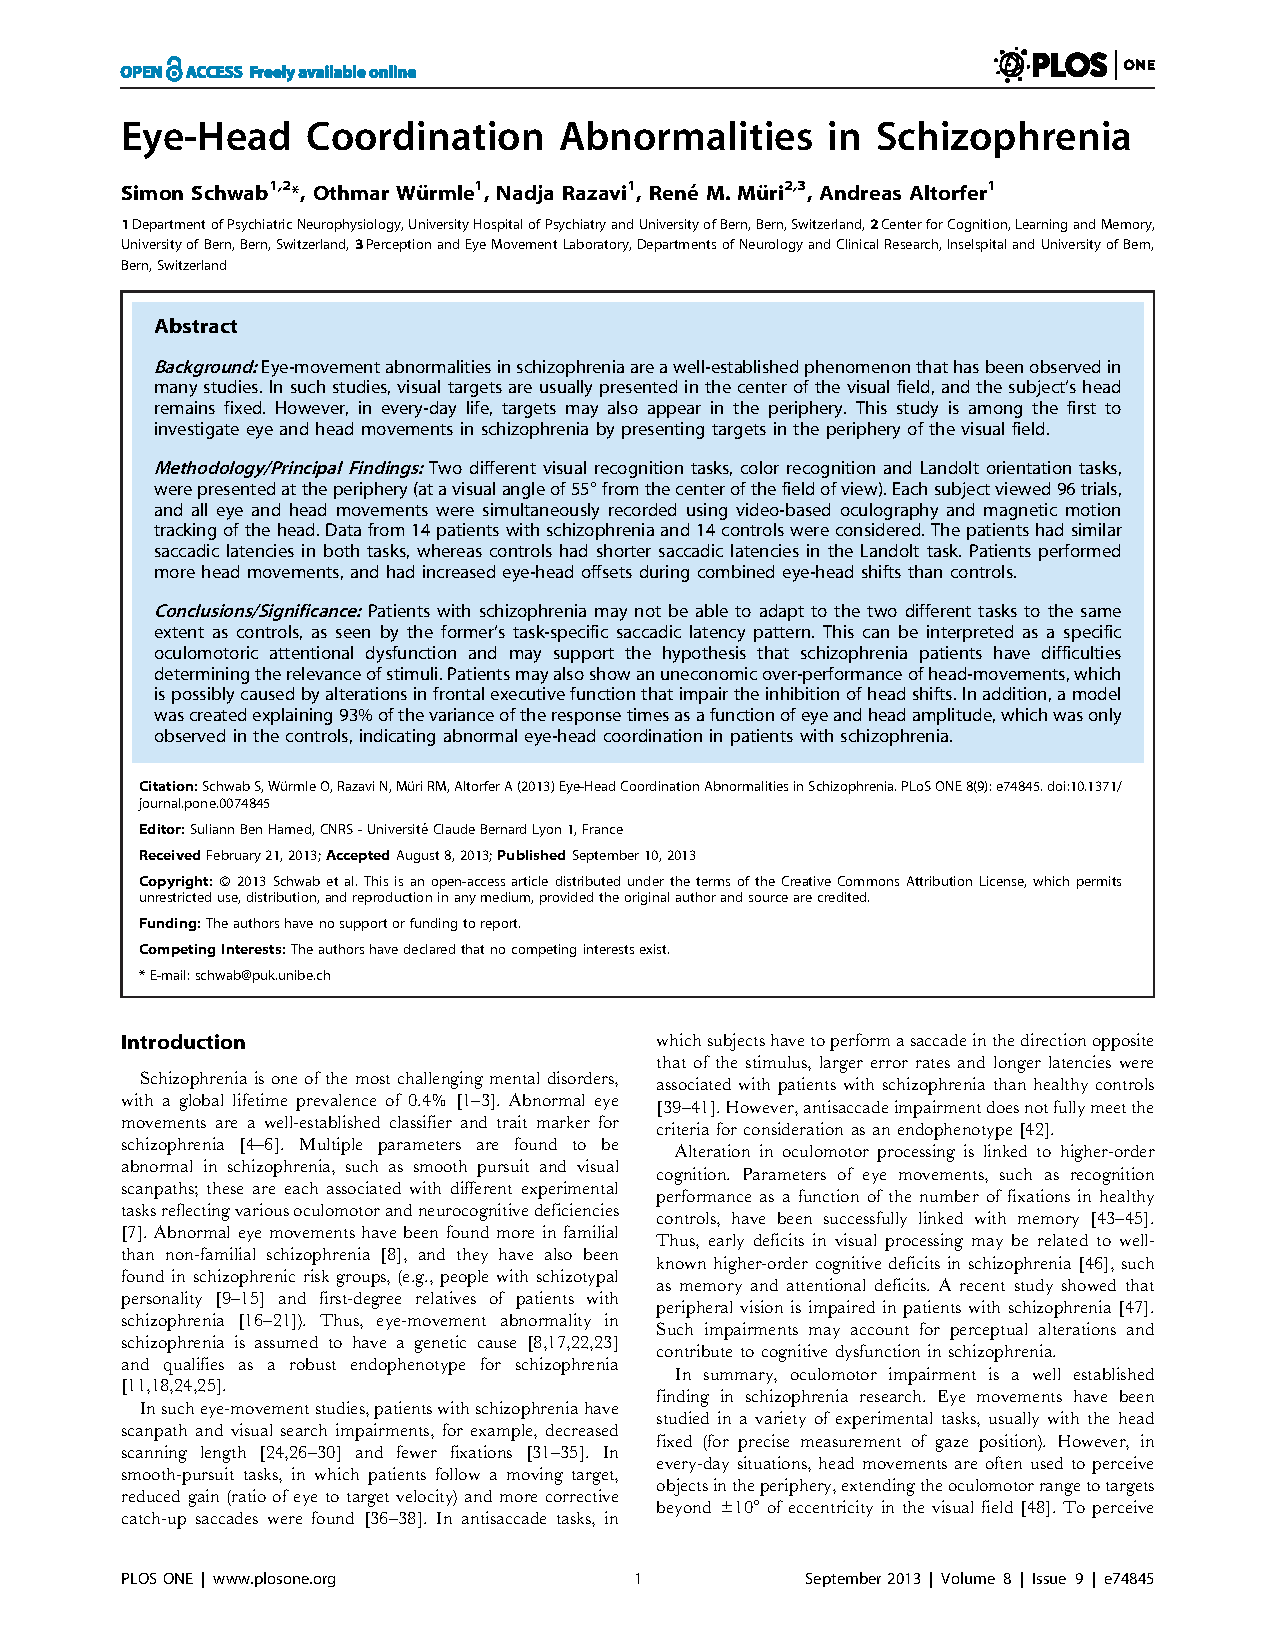
\includepdf[pages=-]{pdf/Schwab2013plosone}

%\chapter{Results}
\label{chap:results}

\section{Eye-head coordination abnormalities in schizophrenia}
\textbf{Schwab, S.}, Würmle, O., Razavi, N., Müri, R.M., \& Altorfer, A. (2013). Eye-head coordination abnormalities in schizophrenia. \textit{PLoS ONE, 8}(9):e74845. doi:10.1371/journal.pone.0074845
%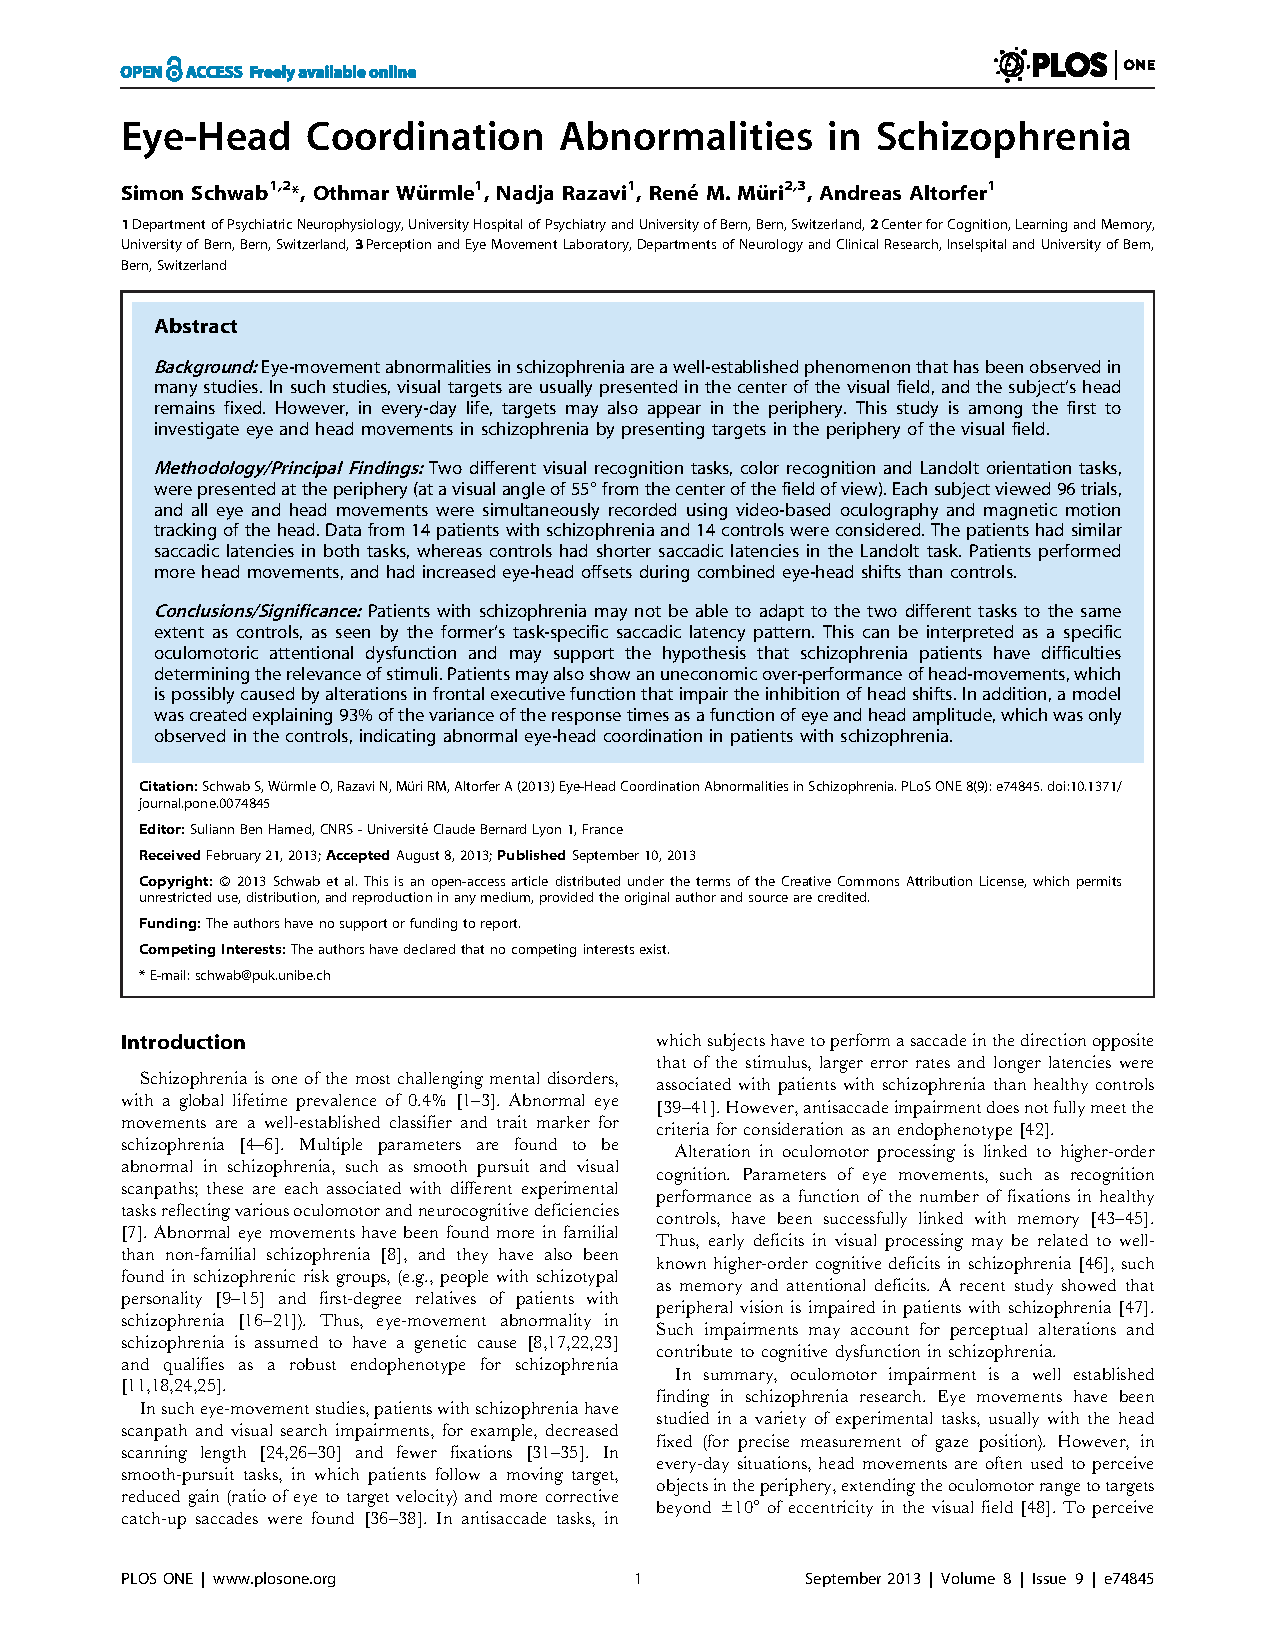
\includepdf[pages=-]{pdf/Schwab2013plosone}

\chapter{Overall Discussion}
\label{chap:discussion}
The main objective of the thesis was to .. \cite{Schwab2013}

\chapter{Perspectives}
\label{chap:perspectives}

The research presented here provided evidence of ...


%\bibliographystyle{IEEEtran}

\bibliography{biblio}
\bibliographystyle{apacite}

%\listoffigures{}
%\listoftables{}

\chapter*{Acknowledgments}
\addcontentsline{toc}{chapter}{Acknowledgments}
First and foremost I want to thank my thesis advisor \textbf{John Doe} ...

\vskip 4em
\hfill L.S.

\chapter*{Curriculum Vitae}
\addcontentsline{toc}{chapter}{Curriculum Vitae}

\section*{Personal}
\textsf{\small
\begin{tabular}{r p{11.7cm}}
%\hline\noalign{\smallskip}
Name          & Luke Skywalker \\
Address       & Department of YX \\
              & Institute \\
              & Street \\
              & City \\
              & Country \\
Phone         & +41 (0)11 111 1111 \\
Email         & \href{mailto:some@mail.com}{\tt some@mail.com} \\
Date of birth  & X \\
Place of birth & X \\
Nationality    & X \\
Place of residence    & X \\
Place of origin& X\\
\end{tabular}
}

\section*{Education}
\textsf{\small
\begin{tabular}{r p{11.7cm}}
%\hline\noalign{\smallskip}
2009 -- 2013    & YX \\
\end{tabular}
}

\section*{Employment}
\textsf{\small
\begin{tabular}{r p{11.7cm}}
%\hline\noalign{\smallskip}
Since 07/2012      & YX \\
\end{tabular}
}

\chapter*{List of Publications}
\addcontentsline{toc}{chapter}{List of Publications}

\section*{Articles published in peer-reviewed journals}
\sffamily

\textbf{Schwab, S.}, Würmle, O., Razavi, N., Müri, R.M., \& Altorfer, A. (2013). Eye-head coordination abnormalities in schizophrenia. \textit{PLoS ONE, 8}(9):e74845. doi:10.1371/journal.pone.0074845

\chapter*{Declaration of Originality}
\addcontentsline{toc}{chapter}{Declaration of Originality}

\large
\sffamily

\textbf{Last name, first name: \hskip 1em Luke Skywalker
\vskip 1em
\noindent Matriculation number: \hskip 1em 00-121-186}
\vskip 6em

\noindent I hereby declare that this thesis represents my original work and that I have used no other sources except as noted by citations.

\noindent All data, tables, figures and text citations which have been reproduced from any other source, including the internet, have been explicitly acknowledged as such.

\noindent I am aware that in case of non-compliance, the Senate is entitled to withdraw the doctorate degree awarded to me on the basis of the present thesis, in accordance with the ``Statut der Universit\"{a}t Bern (Universit\"{a}tsstatut; UniSt)", Art. 69, of 7 June 2011.

\vskip 6em

\noindent Bern, December 5, 2013
\vskip 2em
\noindent Luke Skywalker
\\
%\includegraphics[width=6cm]{eps/signature.eps}


\end{document}
